\documentclass[letterpaper,9pt,twocolumn,twoside,]{pinp}

%% Some pieces required from the pandoc template
\providecommand{\tightlist}{%
  \setlength{\itemsep}{0pt}\setlength{\parskip}{0pt}}

% Use the lineno option to display guide line numbers if required.
% Note that the use of elements such as single-column equations
% may affect the guide line number alignment.

\usepackage[T1]{fontenc}
\usepackage[utf8]{inputenc}

% pinp change: the geometry package layout settings need to be set here, not in pinp.cls
\geometry{layoutsize={0.95588\paperwidth,0.98864\paperheight},%
  layouthoffset=0.02206\paperwidth, layoutvoffset=0.00568\paperheight}

\definecolor{pinpblue}{HTML}{185FAF}  % imagecolorpicker on blue for new R logo
\definecolor{pnasbluetext}{RGB}{101,0,0} %



\title{House Price Prediction using Multiple Regression}

\author[]{Adhip Tanwar, Atharv Natekar, Zhaohui Wang, Yushang Chen
(\href{https://github.sydney.edu.au/atan6081/LAB-07-RE_none_2}{GitHub
Repository})}


\setcounter{secnumdepth}{0}

% Please give the surname of the lead author for the running footer
\leadauthor{}

% Keywords are not mandatory, but authors are strongly encouraged to provide them. If provided, please include two to five keywords, separated by the pipe symbol, e.g:
 \keywords{  House Price Prediction |  Regression Analysis |  Backward
\& Forward AIC  }  

\begin{abstract}
Our investigation explores data collected on houses in Saratoga County,
New York, USA in 2006. Specifically, it aims to understand which
attributes of a house most significantly affect its price. The rationale
for this report is to help aid the housing market in estimating the
house prices as a function of a multivariate analysis. The report fits
the data set into a multiple regression model and conducts a Backward
and Forward search using AIC to find out that the house prices were most
significantly impacted by the living area and by the inclusion of a
waterfront in the property.
\end{abstract}

\dates{This version was compiled on \today} 


% initially we use doi so keep for backwards compatibility
% new name is doi_footer

\pinpfootercontents{YourPackage Vignette}

\begin{document}

% Optional adjustment to line up main text (after abstract) of first page with line numbers, when using both lineno and twocolumn options.
% You should only change this length when you've finalised the article contents.
\verticaladjustment{-2pt}

\maketitle
\thispagestyle{firststyle}
\ifthenelse{\boolean{shortarticle}}{\ifthenelse{\boolean{singlecolumn}}{\abscontentformatted}{\abscontent}}{}

% If your first paragraph (i.e. with the \dropcap) contains a list environment (quote, quotation, theorem, definition, enumerate, itemize...), the line after the list may have some extra indentation. If this is the case, add \parshape=0 to the end of the list environment.


\hypertarget{introduction}{%
\section{Introduction}\label{introduction}}

In the era of globalization, most individuals are focused towards
investing their funds in safe assets. There are several objects that are
often used for such investments, for example, gold, stocks and property.
The property market in particular is one that has observed a constant
increase in value over the years. The average
\href{https://ny.curbed.com/2019/12/13/21009872/nyc-home-value-2010s-manhattan-apartments}{house
prices in Manhattan} for example have steadily increased from
approximately USD 500,000 in 2010 to more than a million dollars in 2019

The decision of purchasing a house is based on multiple factors
including the age of the house, the location, the size, the neighborhood
and various design attributes among the important ones. Since house
prices increase every year, there is a need for a system to predict
house prices in the future. House price prediction can help the
developer determine the selling price of a house. It can also help the
buyers to know the price range of the houses, so they can plan their
finances well.

This research aims to create a house price prediction model using
multiple regression where the house price is considered the dependent
variable and all other variables in the data set are considered the
independent variables. A backward and forward search using alkaline
information criteria (AIC) is used for selection of the most significant
variables in this house price prediction model.

\hypertarget{data-set}{%
\section{Data Set}\label{data-set}}

The given data set -
\href{https://dasl.datadescription.com/datafile/housing-prices-ge19}{\emph{Housing
prices GE19}} - focuses on houses in Saratoga County, New York, USA in
2006. It is a random sample of 1734 houses taken from the full Saratoga
Housing Data (De Veaux). The data set is sourced from
\href{https://rdrr.io/cran/mosaicData/}{\emph{mosaicData}} package in R.
The data was originally collected by Candice Corvetti and used in the
``Stat 101'' case study ``How much is a Fireplace Worth''. The data set
explores 16 variables of interest. \emph{Price} (in US dollars) is our
primary dependent variable under consideration. Apart from that, the
data set contains 3 categorical variables - \emph{heating} (type of
heating system), \emph{fuel} (fuel used for heating), \emph{sewer} (type
of sewer system). The remaining numerical variables in the data set
include \emph{Lot.Size} (in acres), \emph{Age} (age of house in years),
\emph{Land.Value} (in US dollars), \emph{Pct.College} (percent of
neighborhood that graduated college), \emph{Bedrooms},
\emph{Living.Area} (in square feet), \emph{Rooms}, \emph{Bathrooms},
\emph{Fireplaces}, \emph{New.Construct} (whether the property is a new
construction), \emph{Central.Air} (whether the house has central air),
and \emph{Waterfront} (whether property includes waterfront).

\hypertarget{analysis}{%
\section{Analysis}\label{analysis}}

\hypertarget{data-cleaning-transformations}{%
\subsection{Data Cleaning \&
Transformations}\label{data-cleaning-transformations}}

We are analysing the relationship between the house prices and the other
variables in the given data set. Upon initial screening of the data set,
we realised that 3 categorical variables - \emph{Heat.Type} (type of
heating system), \emph{Fuel.Type} (fuel used for heating),
\emph{Sewer.Type} (type of sewer system) - had more than 2
sub-categories. We therefore decided to exclude these variables from our
analysis. Upon conducting linearity checks of the variables in our data
set with the response variable \emph{Price}, we found that by using the
transformation of taking the logarithmic values of \emph{Price},
\emph{Living.Area} and \emph{Land.Value}, we were able to meet the
linearity assumption to a greater extent.

\hypertarget{assumption-testing}{%
\subsection{Assumption Testing}\label{assumption-testing}}

\begin{figure}

{\centering 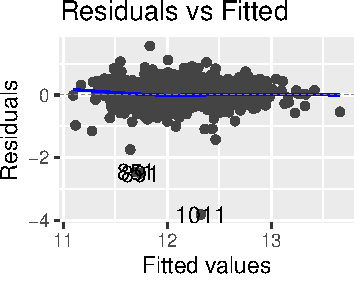
\includegraphics{Executive_Summary_files/figure-latex/fig1-1} 

}

\caption{Residual Plot}\label{fig:fig1}
\end{figure}

\begin{figure}

{\centering 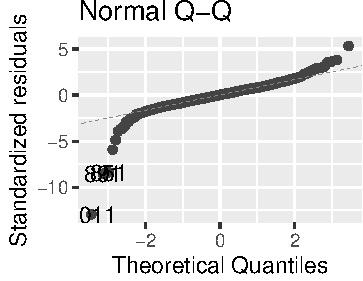
\includegraphics{Executive_Summary_files/figure-latex/fig2-1} 

}

\caption{Q-Q Plot}\label{fig:fig2}
\end{figure}

\begin{itemize}
\tightlist
\item
  \textbf{Homoskedasticity}: In Fig.1 (Residual Plot), no apparent
  fanning out of the residuals over the range of the fitted values can
  be observed. The constant error variance assumption is therefore
  reasonably satisfied
\item
  \textbf{Linearity}: In Fig.1 (Residual Plot), when we look at
  residuals versus fitted values, the blue line is a straight line and
  does not form any distinct pattern (such as a smiley or frowny face).
  Linearity assumption can thus be met.
\item
  \textbf{Independence}: This sample contains 1734 houses, which are
  randomly selected from the Saratoga Housing Data (De Veaux) and
  therefore, the data set can be considered independent.
\item
  \textbf{Normality}: In Fig.2 (Q-Q Plot), most of the points on the QQ
  plot are relatively close to the diagonal line. Barring a few
  outliers, the points seem to fit on the line. Therefore, the data
  seems to be normally distributed.
\end{itemize}

\hypertarget{model-selection}{%
\subsection{Model Selection}\label{model-selection}}

After ensuring that our data set meets the required assumptions, we
proceed towards the final Model Selection.

We first conducted a Backward Search using AIC. Here, we started with a
linear model that contains all the potential explanatory variables and
performed a backward variable selection to remove variables that are not
significant to the data.

We then conducted a Forward Search using AIC. Here, we started with a
model containing no explanatory variables. For each variable in turn, we
investigated the effect of adding the variable from the current model
and only added the variables supplying the most significant information
about our response variable \emph{Price} using the add1() function.

In both the Backward and Forward model, R determines the significance of
each independent variable by performing F-tests and calculating their
p-values.

Finally, we performed a comparison between the model derived using the
forward and backward search. We found out that both these models are
identical and give us the same significant variables, R-Squared values,
and AIC values. We can therefore pick either one of them as our final
model.

\hypertarget{hypothesis-testing}{%
\subsection{Hypothesis Testing}\label{hypothesis-testing}}

\[H_0: \beta_{0} = \beta_{1} = \beta_{2} ... \beta_{10} = 0 \:vs\: H_1: \beta_{i} \neq 0 \:for \:i \in [1,10]\]

For formally testing our hypothesis about the relationship between our
dependent variable \emph{Price} and our derived independent variables
from the final regression model, we set our null hypothesis H0 as all
coefficients of the independent variables (from our regression model)
equal to 0 VS our alternative hypothesis as at least one of these
coefficients not equal to 0.

In order to check our assumptions, we again derived a Residuals Vs
Fitted Values plot and a Q-Q plot on our final model and found out that
both those plots were identical to Fig.1 and Fig.2 (i.e.~the same plots
derived on our full model of all variables). We therefore had strong
evidence for all our assumptions to be reasonably satisfied (the
reasoning explained as above in the Assumption Testing section).

Our Test statistic shows the difference between our full model and our
reduced model after dropping the insignificant variables. The observed
Test Statistic was \textbf{243.2} and P-Value was \textbf{\textless{}
2.2e-16}.

Since the P-Value was less than 0.05, we rejected the null hypothesis,
as we had strong evidence suggesting that there is a significant linear
relationship between Price and the derived independent variables.

\hypertarget{results}{%
\section{Results}\label{results}}

\hypertarget{final-model}{%
\subsection{Final Model}\label{final-model}}

\begin{equation}
  \begin{aligned}
log(Price)&= 6.772 + 0.0344 * Lot Size +\\
       &0.532 * Waterfront - 0.001 * Age + \\
       &0.129 * log(Land Value) - 0.106 * New Construct + \\
       &0.060 * Central Air + 0.530 * log(Living Area) - \\
       &0.002 * Pct.College + 0.106 * Bathrooms + \\
       &0.0126 * Rooms
  \end{aligned}
\end{equation}

\begin{itemize}
\tightlist
\item
  Intercept = 6.772, meaning that considering all attributes of the
  house to be negligible, the logarithmic value of house price will be
  6.772.
\item
  Waterfront has a coefficient of 0.532 which is the biggest coefficient
  in this model, indicating that Waterfront is the \textbf{most
  significant} variable determining the house price.
\item
  Age has a coefficient of 0.001 which is the smallest coefficient in
  this model, indicating that Age of the house (in years) is the
  \textbf{least significant} variable determining the house price.
\end{itemize}

\hypertarget{model-performance}{%
\subsection{Model Performance}\label{model-performance}}

The R-Squared value is 0.585, which means that 58.5\% of the variation
in the logarithmic value of house prices can be explained by the derived
10 independent variables in our final model (from the previous section).

\hypertarget{model-interpretation}{%
\subsection{Model Interpretation}\label{model-interpretation}}

For each of the independent variables and their respective coefficients
derived in our final model, interpretations can be made in the following
manner:

\begin{itemize}
\tightlist
\item
  On average, holding the other variables constant, a 1 unit increase in
  Waterfront leads to a 0.532 unit increase in house prices
\item
  On average, holding the other variables constant, a 1 unit increase in
  Age leads to a 0.001 unit decrease in house prices
\end{itemize}

(Similar format interpretations can be made about each independent
variable in our final model)

\hypertarget{final-discussion}{%
\section{Final Discussion}\label{final-discussion}}

\hypertarget{limitations}{%
\subsection{Limitations}\label{limitations}}

\begin{itemize}
\tightlist
\item
  Some categorical variables such as Heat.Type, Fuel.Type and Sewer.Type
  had to be removed from our analysis since they had more than 2
  sub-categories. The inclusion of those variables could have perhaps
  resulted in a more accurate house price prediction model.
\item
  Our model only explains 58.5\% of the variation in the logarithmic
  value of house prices. This implies that predictions made using this
  model have a reasonable scope of error.
\item
  The given data set only contained infrastructural attributes about
  each individual house. However, house prices also fluctuate heavily by
  exterior factors such as neighborhood, distance from school zones,
  floor number, home loan rates etc. In future research, collection and
  inclusion of data on such external factors could help in forming a far
  more accurate model for predicting house prices.
\end{itemize}

\hypertarget{conclusions}{%
\subsection{Conclusions}\label{conclusions}}

\begin{itemize}
\item
  During our research, we determined that the variables having a
  significant impact on house prices in Saratoga County, New York in
  2006 were Lot Size, Waterfront, Age, Land Value, New Construct,
  Central Air, Living Area, Pct.College, Bathrooms and Rooms.
\item
  Of these variables, the Waterfront and the Living Area variables
  affected the house prices most significantly, whereas the Age and
  Pct.College variables affected the house prices least significantly.
\item
  The model derived in this report only explains 58.5\% of the variation
  in house prices and there is therefore a need to further improve this
  model, which can be done by including data on multiple external
  factors affecting house prices.
\end{itemize}

\hypertarget{references}{%
\section{References}\label{references}}

\begin{itemize}
\item
  Andrews, J. (2019). NYC home prices nearly doubled in the 2010s. What
  do the 2020s hold? Curbed NY.
  \url{https://ny.curbed.com/2019/12/13/21009872/nyc-home-value-2010s-manhattan-apartments}.
\item
  Baptiste Auguie (2017). gridExtra: Miscellaneous Functions for
  ``Grid'' Graphics. R package version 2.3.
  \url{https://CRAN.R-project.org/package=gridExtra}
\item
  David Robinson, Alex Hayes and Simon Couch (2021). broom: Convert
  Statistical Objects into Tidy Tibbles. R package version 0.7.10.
  \url{https://CRAN.R-project.org/package=broom}
\item
  Hadley Wickham, Romain François, Lionel Henry and Kirill Müller
  (2021). dplyr: A Grammar of Data Manipulation. R package version
  1.0.7. \url{https://CRAN.R-project.org/package=dplyr}
\item
  H. Wickham. ggplot2: Elegant Graphics for Data Analysis.
  Springer-Verlag New York, 2016.
\item
  Lüdecke D (2021). \emph{sjPlot: Data Visualization for Statistics in
  Social Science}. R package version 2.8.9, \textless URL:
  \url{https://CRAN.R-project.org/package=sjPlot}\textgreater.
\item
  Max Kuhn (2021). caret: Classification and Regression Training. R
  package version 6.0-90. \url{https://CRAN.R-project.org/package=caret}
\item
  Masaaki Horikoshi and Yuan Tang (2016). ggfortify: Data Visualization
  Tools for Statistical Analysis Results.
  \url{https://CRAN.R-project.org/package=ggfortify}
\item
  Randall Pruim, Daniel Kaplan and Nicholas Horton (2021). mosaicData:
  Project MOSAIC Data Sets. R package version 0.20.2.
  \url{https://CRAN.R-project.org/package=mosaicData}
\item
  Sam Firke (2021). janitor: Simple Tools for Examining and Cleaning
  Dirty Data. R package version 2.1.0.
  \url{https://CRAN.R-project.org/package=janitor}
\item
  Tarr, G (2021). DATA2002 Data Analytics: Learning from Data.
  University of Sydney, Sydney Australia.
\item
  Wickham et al., (2019). Welcome to the tidyverse. Journal of Open
  Source Software, 4(43), 1686,
  \url{https://doi.org/10.21105/joss.01686}
\end{itemize}

%\showmatmethods


\bibliography{pinp}
\bibliographystyle{jss}



\end{document}
